\section{Приложение}

\begin{figure}[h]
    \centering
    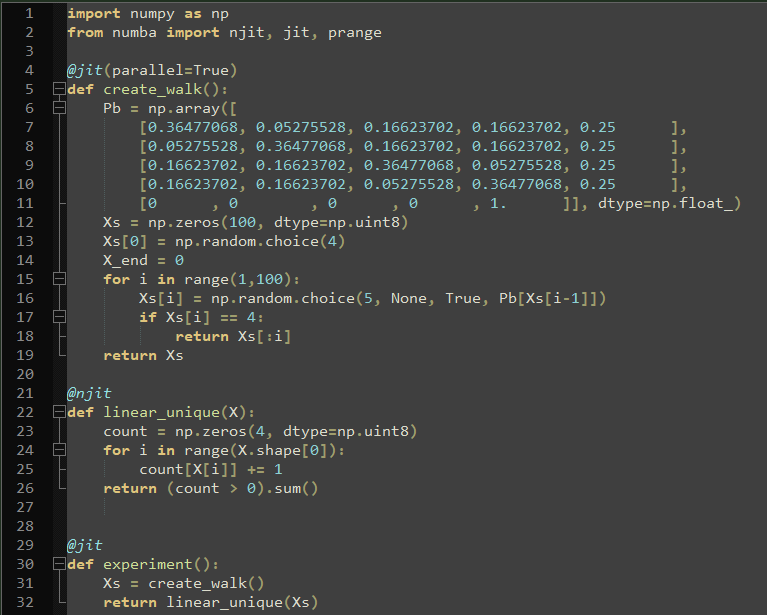
\includegraphics[width=0.8\textwidth]{Sections/Images_2/code_1.png}
    \caption{Исполнительная часть симулирующего кода, подсчитывающая кол-во посещённых точек до достижения начала координат}
    \label{fig:code}
\end{figure}

\begin{table}[h]
    \centering
    \begin{tabular}{|c|c|c|c|c|c|c|}
        \hline
        N & $steps$ & $unique$ & $n_{1}$ & $n_{2}$ & $n_{3}$ & $n_{4}$ \\ \hline
        100 & 7450000 & 0.49(8) & 0.07(3) & 0.33(9) & 0.36(7) & 0.24(9) \\ \hline
        200 & 5684000 & 0.44(7) & 0.05(2) & 0.29(7) & 0.35(5) & 0.30(9) \\ \hline
        500 & 2045000 & 0.39(6) & 0.04(1) & 0.24(5) & 0.34(4) & 0.38(8) \\ \hline
        1000 & 654000 & 0.36(5) & 0.03(1) & 0.22(4) & 0.33(4) & 0.42(7) \\ \hline
        2500 & 132000 & 0.33(4) & 0.027(7) & 0.19(3) & 0.31(3) & 0.48(6)  \\ \hline
        5000 & 37000 & 0.31(4) & 0.024(5) & 0.17(3) & 0.29(3) & 0.51(6) \\ \hline
        10000 & 10000 & 0.29(3) & 0.021(4) & 0.16(2) & 0.28(3) & 0.54(5) \\ \hline
    \end{tabular}
    \caption{Средние доли узлов c 1-4-мя соседями в конформациях модели Rand-Walk длин $10^{2}-10^{4}$}
    \label{tab:Ran_Walk_neigh}
\end{table}

\begin{figure}[]
    \centering
    \caption{Зависимость долей узлов с фиксированным число соседей в случайном блуждании от обратного кол-ва шагов в конформации 1/N}
    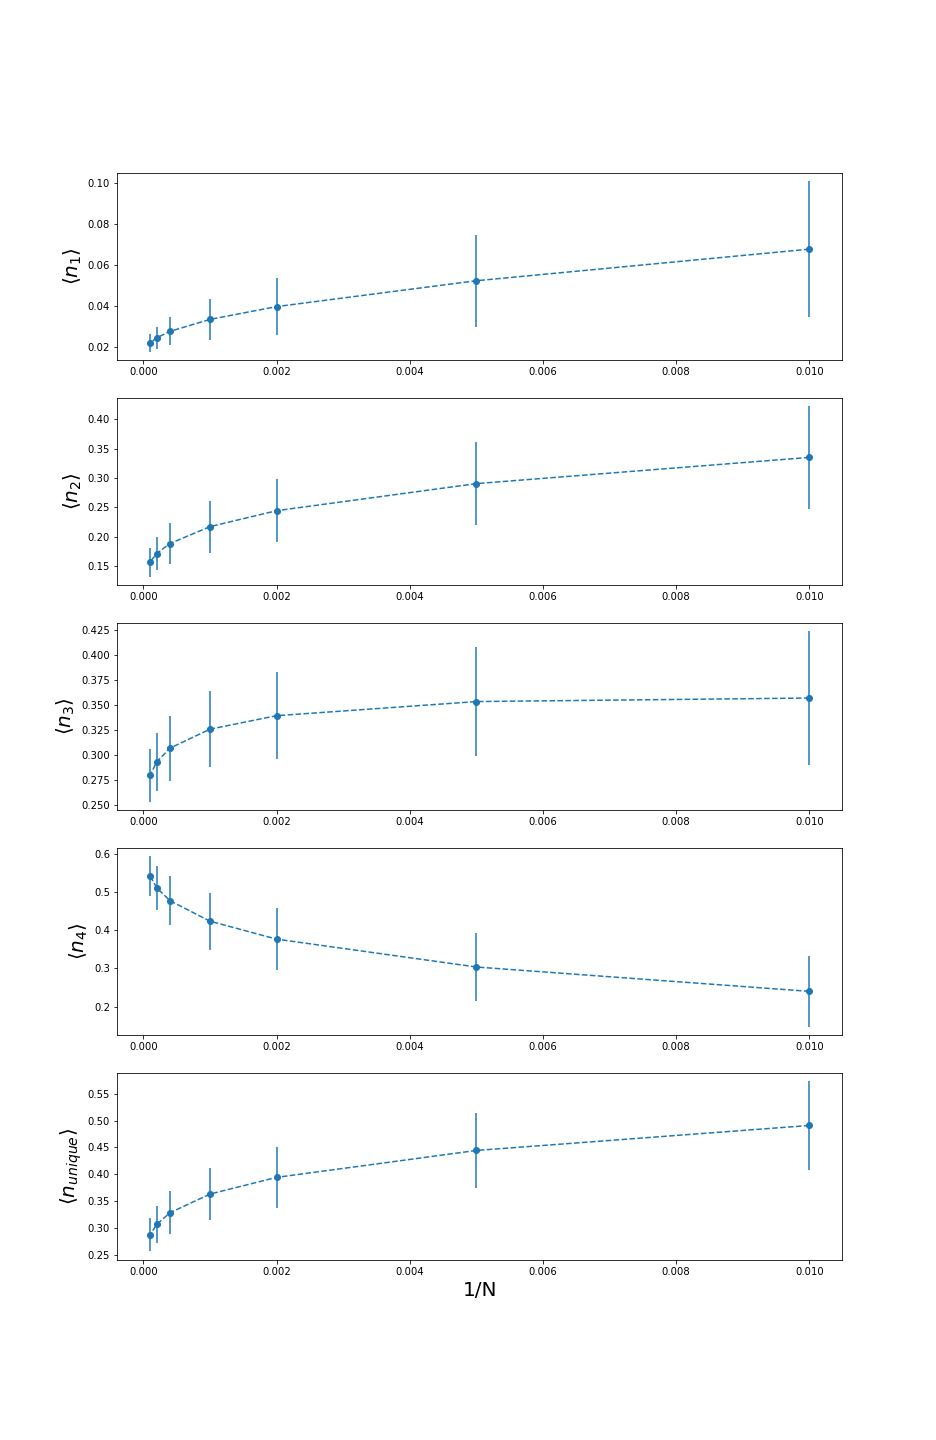
\includegraphics[width=0.9\textwidth]{Sections/Images_2/Rand_Path_N1-4_unique.png}
    \label{fig:Rand_Path_N1_4}
\end{figure}